% !TEX root = main2.tex
\subsection{Experiments on safety verification}
\label{sec:reachexp}

\begin{figure}
	\centering
	\begin{subfigure}[b]{0.45\textwidth}
		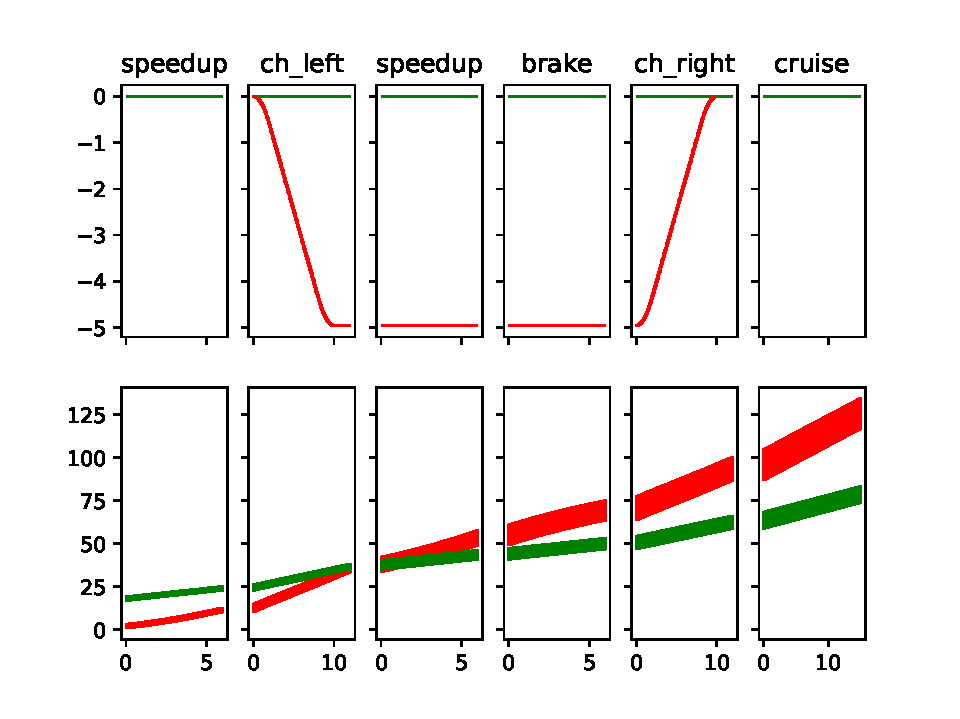
\includegraphics[width=\textwidth,trim={1.0cm 0.8cm 1.5cm 0.8cm},clip]{Car_reachTube.pdf}
		\caption{Safe reachtube. 
			%Initial set is $sy_A\in [0,2], sy_B \in [15,17]$. .
			}
		\label{fig:AutoPassingA}
	\end{subfigure}
	~ ~
	\begin{subfigure}[b]{0.45\textwidth}
		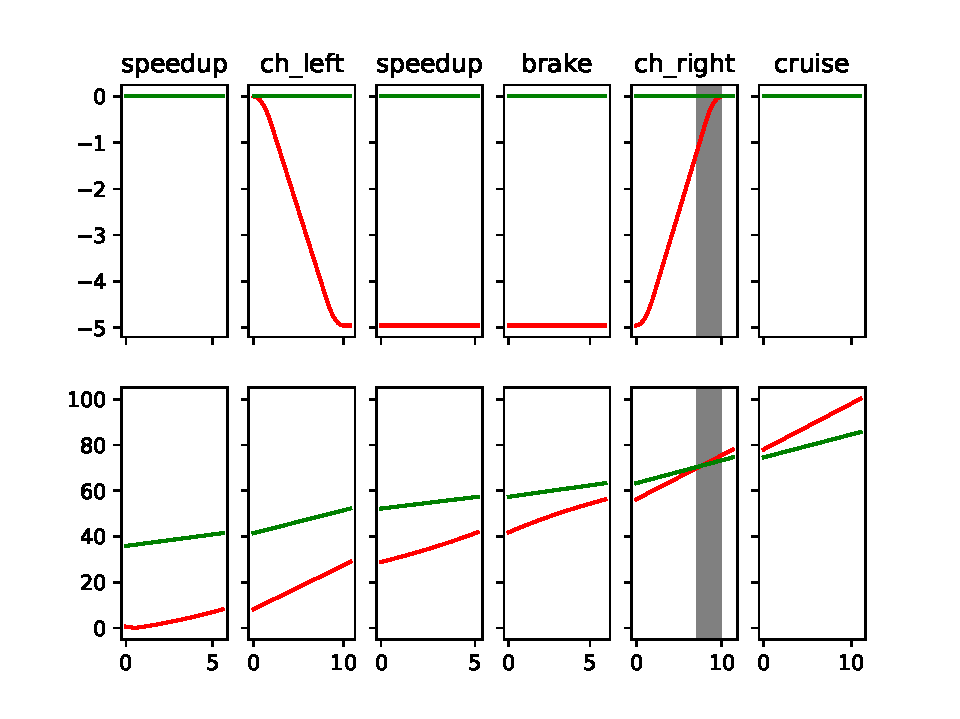
\includegraphics[width=\textwidth,trim={1.0cm 0.8cm 1.5cm 0.8cm},clip]{Car_simulation.pdf}
		\caption{Unsafe execution. 
			%Initial state is $sy_A = 0.5717, sy_B = 35.89$.
			%Top:  $sx_A,sx_B$. 
			%Bottom: $sy_A, sy_B$.
			}
		\label{fig:AutoPassingB}
	\end{subfigure}
\vspace{-8pt}
\caption{\small $\auto{AutoPassing}$  verification. Vehicle A's (red) modes are shown above each subplot. Vehicle B (green) is in \Lmode{cruise}. 
	Top: $sx_A,sx_B$. Bottom: $sy_A, sy_B$.
	%Unsafe set is that the relative distance between A and B in both directions is less than $2$.
	 }
\label{fig:AutoPassing}
\end{figure}

The algorithms have been implemented in {\toolname} and
have been used to automatically verify the benchmarks from
Section~\ref{sec:prelims} and an Automatic Transmission System (Appendix~\ref{ssec:gear}). 
%
The transition graph, the initial set, and unsafe set are given in a text file. {\toolname} uses simulators for modes, and outputs either ``Safe'' of ``Unsafe''. Reachtubes or counter-examples computed during the analysis are also stored in text files.

The implementation is in Python using the MatLab's Python API for accessing the \Simulink ~simulators. Py-GLPK~\cite{python-glpk-package} is used to find the
parameters of discrepancy functions;
%
either global (GED) or piece-wise (PED) discrepancy can be selected by
the user.  Z3~\cite{de2008z3} is used for reachtube operations.
%\chuchu{
	At this stage, all the benchmarks we are working on heavily
  rely on {\Mathworks} {\Simulink}. We don't have a public
  {\Mathworks} license to release the tool, and it is complicated for
  the users to build a connection between {\toolname} and
  their own {\Simulink} models. We will release {\toolname} soon after
  we move the blackbox benchmarks to a different open source software.
  %}

Figure~\ref{fig:AutoPassing} shows example plots of computed safe
reachtubes and counter-examples for a simplified
$\auto{AutoPassing}$ in which vehicle B stays in the \Lmode{cruise} always.
%\mitras{why? change the example in the ealier section to fit this. I dont think this examples appears anywhere else.}
As before, vehicle A goes through a sequence of  modes %sequence \Lmode{ch\_left}, \Lmode{speedup},\Lmode{brake}, and  \Lmode{ch\_right}, \Lmode{cruise} over specified time intervals 
to overtake B. 
%\mitras{Relate x and y axes to direction of lane, left-right lanes.}
Initially, for both $i \in \{A,B\}$, $sx_i = vx_i = 0$ and $vy_i = 1$, i.e., both are cruising at constant speed at the center of the right lane; initial positions along the lane are $sy_A\in [0,2], sy_B \in
[15,17]$.  Figure~\ref{fig:AutoPassingA} shows the lateral positions
($sx_A$ in red and $sx_B$ in green, in the top subplot), and the
positions along the lane ($sy_A$ in red and $sy_B$ in green, in the
bottom plot).
 Vehicle A moves to left lane ($sx$ decreases) and then
back to the right, while B remains in the right lane, as A overtakes
B (bottom plot).  The unsafe set $(|sx_A-sx_B|<2 \ \&\ |sy_A-sy_B|<2)$ is proved to be disjoint from computed reachtube.  With a different
initial set, $sy_B \in [30,40]$, \toolname\ finds counter-example (Figure~\ref{fig:AutoPassingB}).

%\begin{table}
%\begin{tabular}{ll}
%$\U_{p1}$ & \makecell{Powerup:$t>4.4 \& \lambda \in [12.4,12.6]$ \\ Normal:$t>4.4 \& lambda \in [14.6,14.8]$}\\
%$\U_{p2}$ & \makecell{Powerup:$t>1.2\& \lambda \in [12.4,12.6]$ \\ Normal:$t>1.2 \& lambda \in [14.6,14.8]$}\\
%$\U_{c1}$ & \makecell { Allmode:relative dis between \\ two cars for both direction $<2$} \\
%$\U_{c2}$ & \makecell { Allmode:relative dist between \\ any two cars for both direction $<2$} \\
%$\U_{t1}$ & Allmode:Enginerpm $\in [0,4000]$\\
%$\U_{t2}$ & Allmode:Enginerpm $\in [0,3000]$\\
%\end{tabular}
%\end{table}


% Table generated by Excel2LaTeX from sheet 'Sheet1'
\begin{table}
\begin{center}
  \centering
\resizebox{\columnwidth}{!}{%
    \begin{tabular}{|c|rlcccr|}
    \hline
    Model &  TH &  Initial set & $\U$ & Ref & Safe & Runtime  \\
    \hline
    \makecell[c]{$\auto{Powertrn}$ \\ (5 vers, 6 edges)}   & 80    & \makecell[l]{$\lambda \in [14.6,14.8]$} & $\U_{p}$      & 2     & \cmark & 217.4s \\
\cline{1-7}
      %  & 80    & Same as above & $\U_{p2}$    & 0     & \xmark & 39.2s \\ \hline
    {$\auto{AutoPassing}$}   & 50    & $sy_A \in [-1,1]$ $sy_B \in [14,16]$ & $\U_{c}$    & 4     & \cmark  & 208.4s \\ \cline{2-7}
     (12 vers, 13 edges) & 50    &  $sy_A \in [-1,1]$ $sy_B \in [4,6.5]$ & $\U_{c}$     & 5     & \xmark & 152.5s \\ \hline
    {$\auto{Merge}$ } &   50    & $sx_A \in [-5,5]$ $sy_B\in [-2,2]$ & $\U_{c}$      & 0     & \cmark  & 55.0s \\ \cline{2-7}
     (7 vers, 7 edges) &   50    &  $sx_A \in [-5,5]$  $sy_B \in [2,10]$ & $\U_{c}$      & -     & \xmark & 38.7s \\ \hline
    {$\auto{Merge3}$} &   50    &  \makecell[l]{$sy_A \in [-3,3]$ $sy_B \in [14, 23]$\\$sy_C \in [36, 45]$} & $\U_{c}$      & 4     & \cmark  & 197.6s \\ \cline{2-7}
     (6 vers, 5 edges) &   50    & \makecell[l]{$sy_A \in [-3,3]$ $sy_B \in [14,15]$ \\ $sy_C \in [16, 20]$} & $\U_{c}$     & -     & \xmark & 21.3s \\ \hline
   \makecell[c]{ {$\auto{ATS}$ }\\ (4 vers, 3 edges)} &  50    & Erpm $\in [900,1000]$& $\U_{t}$    & 2     & \cmark  & 109.2s \\ \cline{2-7}
      %&  350   & Same as above & $\U_{t2}$   & 0     & \xmark & 31.1s \\
    \hline
    \end{tabular}%
}
\vspace{-14pt}
  \caption{\small Safety verification results. Numbers below benchmark names: \# vertices and edges of $G$, TH: duration of shortest path in $G$,  Ref: \# refinements performed; Runtime: overall running time.}
\label{table:results}
  \end{center}
\end{table}%

Table~\ref{table:results} summarizes some of the verification results obtained using \toolname. $\auto{ATS}$ is an automatic
transmission control system (see Appendix~\ref{ssec:gear} for more details). These experiments were
performed on a laptop with Intel Core i7-6600U CPU and 16 GB RAM. 
%For each benchmark, the size of the graph is given in parentheses. 
%The
%time horizon (TH) is the maximum time up to which reachtubes extend.
%
The initial range of only the salient continuous variables are shown in the table.  The unsafe sets are discussed with the model description. For example $\U_c$ means  two vehicles are too close.
%
%The number of (edge or initial set) refinements performed is reported in column $Ref$.
%
For all the benchmarks, the algorithm terminated in a few minutes which includes the time to simulate, learn discrepancy, generate reachtubes, check the safety of the reachtube, over all refinements.

%\mitras{Chuchu: more on the implementation details, platform used for this set of experiments.}
%
 For the results presented in Table~\ref{table:results}, we used GED. The reachtube generated by PED for $\auto{Powertrn}$ is more precise, but for the rest, the reachtubes and the verification times using both GED and PED were comparable.  
%
%Table ~\ref{table:results} contains powertrain control system ($\auto{Powertrn}$), ADAS ($\auto{AutoPassing}$, $\auto{Merge}$, $\auto{3Merge}$) and automatic transmission control (ATS). 
%
%
%safe and/or unsafe cases by changing initial set or unsafe set. 
%The initial values not shown up in the tables are
%\begin{inparaenum} [1)]
%\item $\auto{Powertrn}$: $p \in [0.6115,0.6315], pe \in [0.5555,0.5755], i \in [0,0.01]$; 
%\item $\auto{AutoPassing}$, $\auto{Merge}$, $\auto{3Merge}$: $\forall i = A,B$, if not mentioned in the "Initial set" column of the table, $sx_i = sy_i = 0, vx_i = vy_i = 1$;
%\item ATS: $v=0, T_i = 394.05, T_o = 52.92,$ Trpm $= 0$.
%\end{inparaenum}
%
%
%
%The unsafe sets are defined as:
%\begin{inparaenum} [1)]
%\item $\U_{p1}$: in \Lmode{powerup} mode, $t>4.4 \& \lambda \in [12.4,12.6]$, in \Lmode{normal} mode, $t>4.4 \& lambda \in [14.6,14.8]$; 
%\item $\U_{p2}$: in \Lmode{powerup} mode, $t>1.2\& \lambda \in [12.4,12.6]$, in \Lmode{normal} mode, $t>1.2 \& lambda \in [14.6,14.8]$;
%\item $\U_{c1}$: in all modes, relative distances on both $x,y$ axises between two cars $<2$;
%\item $\U_{c2}$: in all modes, relative distances on both $x,y$ axises between any two cars $<2$;
%\item $\U_{t1}$: in all modes, Erpm $\in [0,4000]$;
%\item $\U_{t2}$: in all modes, Erpm $\in [0,3000]$.
%\end{inparaenum}
%
In addition to the $\mathit{VerifySafety}$ algorithm, \toolname\ also
looks for counter-examples by quickly generating random executions of
the hybrid system.  If any of these executions is found to be unsafe,
\toolname\ will return ``Unsafe'' without starting the
$\mathit{VerifySafety}$ algorithm.
%simulation traces for the entire graph to capture counter examples. The simulation traces are from random positions of the initial set, and will transit from one mode to another at random time within the transition time defined by the edge label. If any simulation trace violates the safety requirement, the algorithm will return "unsafe" with the counter example trace. 
%If all such simulations are safe, then it proceeds with $\mathit{VerifySafety}$.
%In our experiments, this strategy found counter-examples quickly. 
% is generally faster to find counter-examples than proving safety since once a counter example is found, the algorithm will terminate and return unsafe. However, The algorithm may need a few refinement before it can prove the system is safe for any initial condition in the initial set and uncertainty in the transition time.

%\newpage
%% !TEX root = main2.tex
\subsection{Experiments on trace containment reasoning}
\label{sec: sub_exp}
%We describe two experiments illustrating applications of the above results. 

\paragraph{Graph simulation}
Consider the $\auto{AEB}$ system of Section~\ref{ssec:adas} with the
scenario where Vehicle B is stopped ahead of vehicle A, and A transits
from \Lmode{cruise} to \Lmode{em\_brake} to avoid colliding with B.
In the actual system ($G_2$ of Figure~\ref{fig: em_brake_graphs}), two different sensor systems
trigger the obstacle detection and emergency braking at time intervals
$[1,2]$ and $[2.5,3.5]$ and take the system from vertex $0$
(\Lmode{cruise}) to two different vertices labeled with
\Lmode{em\_brake}.

\begin{figure}[ht]
    \begin{subfigure}[b]{0.3\textwidth}
        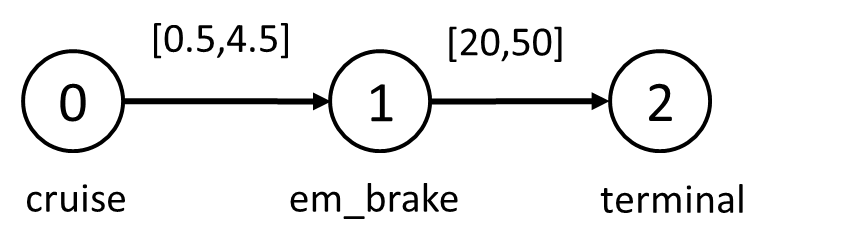
\includegraphics[width=\textwidth]{brake_2_modes.png}
        \caption{\small Transition graph $G_1$.}
        \label{fig: em_brake_graphsA}
    \end{subfigure}
    \begin{subfigure}[b]{0.3\textwidth}
        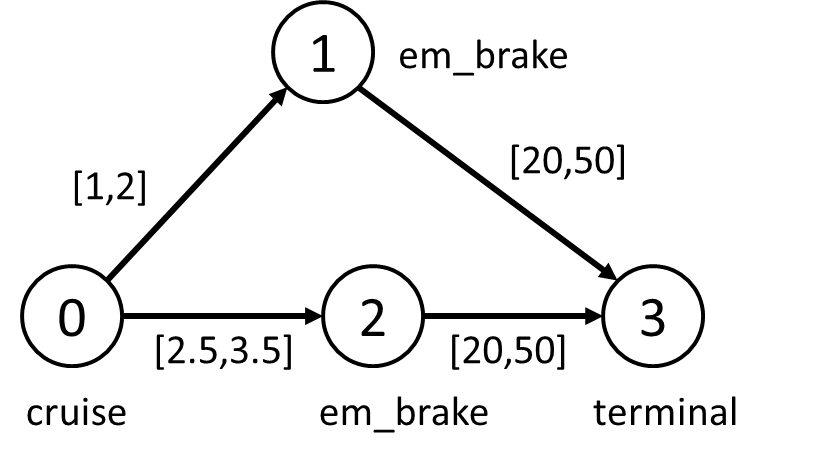
\includegraphics[width=\textwidth]{brake_3_modes.png}
        \caption{Transition graph $G_2$.}
        \label{fig: em_brake_graphsB}
    \end{subfigure}
    \begin{subfigure}[b]{0.35\textwidth}
	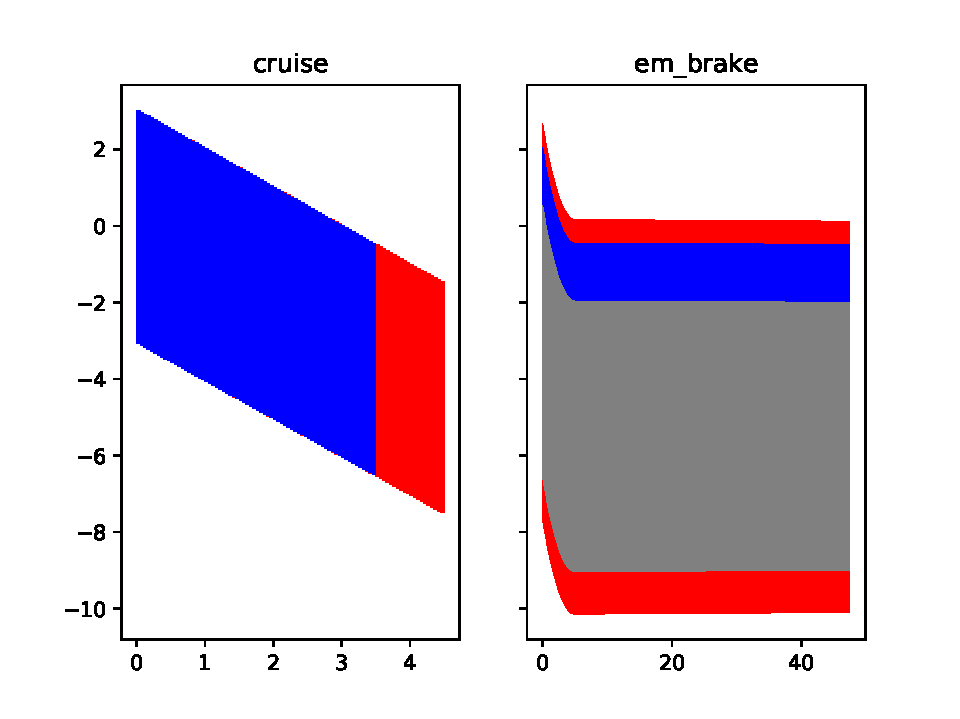
\includegraphics[width=\textwidth]{Abstraction_reachTube.pdf}
	\caption{$\auto{AEB}$ Reachtubes.}
	%\caption{Reachtubes of graphs in Figure \ref{fig: em_brake_graphs}. Red tubes corresponds to Figure \ref{fig: em_brake_graphsA}, blue and gray tubes corresonds to Figure \ref{fig: em_brake_graphsB}}
	\label{fig:abstraction}
    \end{subfigure}
\caption{\small Graphs and reachtubes for the Automatic Emergency Braking $\auto{AEB}$ system.}
\label{fig: em_brake_graphs}
\end{figure}

%
To illustrate trace containment reasoning, consider a simpler
graph $G_1$ that allows a single transition of A from \Lmode{cruise}
to \Lmode{em\_brake} over the interval bigger $[0.5, 4.5]$. Using
Proposition~\ref{prop:hybrid-contain} and checking that graph $G_2
\preceq_{\sf id} G_1$, it follows that verifying the safety of
$\auto{AEB}$ with $G_1$ is adequate to infer the safety with $G_2$.
Figure~\ref{fig:abstraction} shows that the safe reachtubes returned
by the algorithm for $G_1$ in red, indeed contain the reachtubes for
$G_2$ (in blue and gray).
%The graphs of the system, along with the reachtube plots are provided in the Appendix.
%For more complex graphs  

%Figure \ref{fig: em_brake_graphs} shows two different graphs specifying two scenarios.  
%Figure \ref{fig: em_brake_graphsA} shows that vehicle A could transit from \Lmode{cruise} to \Lmode{em\_brack} within $[0.5, 4.5]$. However, in  Figure \ref{fig: em_brake_graphsB} the transition may happen in two disjoint time intervals $[1,2],[2.5,3.5]$. 

%Since both the vehicles never change the lane, we will only consider variables along the $y$ coordinate. The initial set is $sy_A \in [-3,3], sy_B \in [14,23], vy_A = 1, vy_B =0$. The unsafe set is set to be $|sy_A-sy_B| < 2$ ($|sx_A-sx_B| < 2$ is always satisfied).

% In the \Lmode{cruise} mode, the red tube corresponds to the vertex $0$'s reachtube in Figure~\ref{fig: em_brake_graphsA} and the blue one corresponds to vertex $0$ in Figure \ref{fig: em_brake_graphsB}. Similarly, in the \Lmode{em\_brake}, the red tube corresponds to the vertex $0$'s reachtube in Figure \ref{fig: em_brake_graphsA}, the blue tube corresponds to the vertex $1$'s reachtube in Figure \ref{fig: em_brake_graphsB} and the gray tube corresponds to the vertex $2$'s reachtube in Figure \ref{fig: em_brake_graphsB}. It can be clearly seen from Figure \ref{fig:abstraction} that in both modes,  the reachtubes of Figure \ref{fig: em_brake_graphsB} is contained in the reachtube of Figure \ref{fig: em_brake_graphsA}, which is consistent with proposition \ref{prop:hybrid-contain}.


\vspace{-10pt}
\paragraph{Sequential composition}
We revisit the $\auto{Powertrn}$ example of
Section~\ref{ex:powertrain}. The initial set $\Theta$ and unsafe set
are the same as in Table \ref{table:results}.  Let $G_A$ be the graph
($v_0$,\Lmode{startup}) $\xrightarrow{[5,10]}$ ($v_1$,\Lmode{normal})
$\xrightarrow{[10,15]}$ ($v_2$,\Lmode{powerup}), and $G_B$ be the
graph ($v_0$,\Lmode{powerup}) $\xrightarrow{[5,10]}$
($v_1$,\Lmode{normal}) $\xrightarrow{[10,15]}$
($v_2$,\Lmode{powerup}).  The graph $G_1 =$ ($v_0$,\Lmode{startup})
$\xrightarrow{[5,10]}$ ($v_1$,\Lmode{normal}) $\xrightarrow{[10,15]}$
($v_2$,\Lmode{powerup}) $\xrightarrow{[5,10]}$ ($v_3$,\Lmode{normal})
$\xrightarrow{[10,15]}$ ($v_4, $\Lmode{powerup}), can be expressed as
the composition $G_1 = G_A \seqcomp G_B$. Consider the two hybrid
systems $\H_i = \langle \L, \Theta_i, G_i, \TL \rangle$, $i \in
\{A,B\}$ with $\Theta_A = \Theta$ and $\Theta_B =
\reach{\H_A}^{v_2}$. {\toolname}'s estimate of $\Theta_{B}$ had
$\lambda$ in the range from $14.68$ to $14.71$. The reachset
$\reach{\H_B}^{v_2}$ computed by {\toolname} had $\lambda$ from
$14.69$ to $14.70$. The remaining variables also were observed to
satisfy the containment condition. Therefore, $\reach{\H_B}^{v_2}
\subseteq \Theta_{B}$.  Consider the two hybrid systems $\H_i =
\langle \L, \Theta, G_i, \TL \rangle$, $i \in \{1,2\}$, where $G_1$ is
(defined above) $ G_A \seqcomp G_B$, and $G_2 = G_A \seqcomp G_B
\seqcomp G_B \seqcomp G_B$.  Using Theorem
\ref{thm:seqcomp-mainresult} it suffices to analyze $\H_1$ to verify
$\H_2$.  $\H_1$ was been proved to be safe by \toolname\ without any
refinement.  As a sanity check, we also verified the safety of $\H_2$.
%is \Lmode{normal} $\xrightarrow{[10,15]}$ \Lmode{powerup} $\xrightarrow{[5,10]}$ \Lmode{normal} $\xrightarrow{[10,15]}$ \Lmode{term} $\xrightarrow{[0,0]}$ \Lmode{powerup} $\xrightarrow{[5,10]}$ \Lmode{normal} $\xrightarrow{[10,15]}$ %\Lmode{term} $\xrightarrow{[0,0]}$ \Lmode{powerup} $\xrightarrow{[5,10]}$ \Lmode{normal} $\xrightarrow{[10,15]}$ \Lmode{term}. 
{\toolname} proved $\H_2$ safe without any refinement as well.

%\input{sequential_exp}
